\section{Model}
\label{sec:model}
\addcontentsline{toc}{chapter}{Model}

We model very simple robots like in \cite{butler02}, we call them bots. Furthermore there are
obstacles, which provide the bots a surface to stand on, and boxes, which can be
pushed around. The bots, as we call them, are able to move around a surface,
climb up each other and small obstacles, and to push boxes around. The goal of
the bots is to push a box over a surface with a gap. They can do this by filling
the gap with bots to supply a surface to push the box over.

This is modelled in a 2 dimensional cellular automata. There is gravity
applied to boxes and bots in the downward direction and bots push boxes to the
right, as specified in section \ref{sec:world}. The movement of the bots is
determined by cellular automata rules, which are specified in section
\ref{sec:ca-rules}.


\subsection{The world}
\label{sec:world}
Boxes and bots fall down immediately if they are not supported by a box, bot or
obstacle under it. The world is initialised with a floor of obstacles on the
bottom, to prevent bots from falling out of the world. On top of the first layer
of obstacles is another layer with an single optional gap in it with an integer
length between 1 and 10.

If a bot  has a box to it's right it immediately and automatically pushes the box to the
right, if possible. A box has a integer weight between 1 and 10. Bots can work
together pushing a box if they are in a line left of a box. If the length of
this line is equal or longer than the combined weight of a line of boxes lying
to the right of the bots the boxes get pushed one square to the right. Bots
never push a box in a gap, and also never push boxes that have something on top
of them.

\subsection{Cellular Automata}
\label{sec:ca-rules}
The bots move according to cellular automata rules, which are presented in figure
\ref{fig:ca-rules}. Bots get randomly selected to activate. There is particular
order the bots activate in, and a bot can not activate at all in a time
span while another bot gets activated multiple times. If a bot activates it tries
to apply a cellular automate rule. The rules are applied in order, the first one
that matches gets executed.

%Maybe say something about that all the rules can activate when there is another
%bot on top. And about bots jumping down arbitrary distances if they are on top
%of a box.

\begin{figure}

\subfloat[Rule 1]{
    \label{fig:ca-rules:1}
    \begin{minipage}[b]{0.3\linewidth}
    \centering
    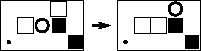
\includegraphics[scale=1.2]{images/rule1}
    \end{minipage}
}%
\hfill
\subfloat[Rule 2a]{
    \label{fig:ca-rules:2a}
    \begin{minipage}[b]{0.3\linewidth}
    \centering
    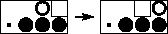
\includegraphics[scale=1.2]{images/rule2a}
    \end{minipage}
}%
\hfill
\subfloat[Rule 2b]{
    \label{fig:ca-rules:2b}
    \begin{minipage}[b]{0.3\linewidth}
    \centering
    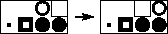
\includegraphics[scale=1.2]{images/rule2b}
    \end{minipage}
}

\subfloat[Rule 3]{
    \label{fig:ca-rules:3}
    \begin{minipage}[b]{0.3\linewidth}
    \centering
    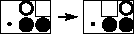
\includegraphics[scale=1.2]{images/rule3}
    \end{minipage}
}%
\hfill
\subfloat[Rule 4]{
    \label{fig:ca-rules:4}
    \begin{minipage}[b]{0.3\linewidth}
    \centering
    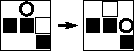
\includegraphics[scale=1.2]{images/rule4}
    \end{minipage}
}%
\hfill
\subfloat[Rule 5a]{
    \label{fig:ca-rules:5a}
    \begin{minipage}[b]{0.3\linewidth}
    \centering
    
\includegraphics[scale=1.2]{images/rule5a}
    \end{minipage}
}

\subfloat[Rule 5b]{
    \label{fig:ca-rules:5b}
    \begin{minipage}[b]{0.3\linewidth}
    \centering
    
\includegraphics[scale=1.2]{images/rule5b}
    \end{minipage}
}%
\hfill
\subfloat[Rule 6]{
    \label{fig:ca-rules:6}
    \begin{minipage}[b]{0.3\linewidth}
    \centering
    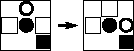
\includegraphics[scale=1.2]{images/rule6}
    \end{minipage}
}%
\hfill
\subfloat[Rule 7]{
    \label{fig:ca-rules:7}
    \begin{minipage}[b]{0.3\linewidth}
    \centering
    
\includegraphics[scale=1.2]{images/rule7}
    \end{minipage}
}

\subfloat[]{
    \begin{minipage}[b]{\linewidth}
    \centering
    Active Bot: 
\includegraphics[scale=1.2]{images/bot-active}\quad
    Bot: 
\includegraphics[scale=1.2]{images/bot}\quad%
    Obstacle: 
\includegraphics[scale=1.2]{images/obstacle}\quad%
    Box: 
\includegraphics[scale=1.2]{images/box}\quad

    Empty space: 
\includegraphics[scale=1.2]{images/empty}\quad%
    Bot, Obstacle or Box: 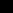
\includegraphics[scale=1.2]{images/some-turtle}\quad%
    No bot: 
\includegraphics[scale=1.2]{images/no-bot}\quad%
    \end{minipage}
}
\caption{Cellular automata rules for moving bots.}
\label{fig:ca-rules}
\end{figure}
